\section{Comparaison avec la photo avec un
crop}\label{comparaison-avec-la-photo-avec-un-crop}

\begin{figure}[htbp]
\centering
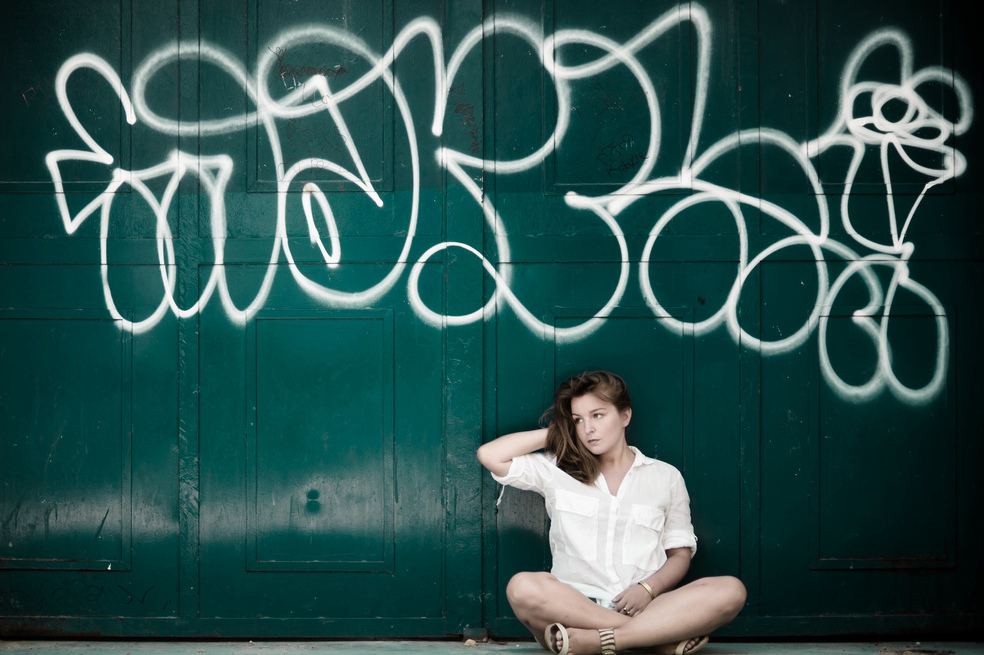
\includegraphics{../../photos/crop.jpg}
\caption{Photo crop}
\end{figure}

\begin{table}[htbp]
\centering
\begin{tabular}{llr}
\bfseries Formes &
\bfseries Bhattacharyya (\%)%
\DTLforeach*[\DTLiseq{\fichier}{photos/crop.jpg}]{valeurs}{%
\fichier=Fichier, \formes=Formes,\bhatta=Bhattacharyya}{%
\\
\formes & \bhatta}
\end{tabular}
\end{table}


\emph{Le crop est un procédé qui consiste à recadrer une photo}

La comparaison de la photo originale avec la photo à laquelle nous avons
appliqué un crop nous montre une différence très faible au niveau de la
couleur ($0.27 \%$ de différence par le filtre de Bhattacharyya) contre
une différenciation prononcée au niveau des formes ($51.16 \%$ avec la
comparaison en Sobel). \\
Cela s'explique par le fait qu'un crop est un redécoupage de la photo et qu
donc certaines formes délimitables grâce au filtre de Sobel ne sont plus
présentes sur la photo. Cependant les couleurs ne changent pas ce qui explique
ce pourcentage de différence très faible au niveau colorimétrique.